\chapter{Kinematic reweighting in strong-production analysis}
\label{app:meffrw}

In this appendix we discuss in more details the kinematic reweighting mentioned in Section \ref{sec:strong:dataMC},
designed to mitigate the effect of the mismodelling that affects all the energy-related variables in the 1-lepton channel,
where we observe a downward trend in the data/MC ratio, clearly visible e.g. in the bottom panel of 
Figure \ref{fig:strong:datamc:meff_prerw_1L}; this is not present in the 0-lepton channel, as can be seen in 
Figure \ref{fig:strong:datamc:meff_prerw_0L}.
This difference in trends is problematic for the analysis, since all of the \glspl{vr} require at least one signal lepton, 
including the ones used to derive the prediction for 0-lepton \glspl{sr}.

To have a better estimate of the background in the high-$\meff$ regime, a reweighting has been derived to bring the MC prediction closer to the observed data. This reweighting is computed in a region that requires:
\begin{itemize}
\item At least one lepton,
\item $\met$ $>$ 200 GeV,
\item exactly 2 b-jets,
\item $\mtb$ $<$ 140 GeV.
\end{itemize}

This selection is orthogonal to \glspl{sr} and \glspl{cr} but has a similar background composition. 
The $\mtb$ selection reduces further the signal contamination and allows for a validation region with exactly 2 b-jets and high $\mtb$. 
The same trend in the ration data/MC in the \meff distribution has been observed also in other regions non $\ttbar$-domninated,
therefore the reweighting is computed taking into account all backgrounds and applied to all backgrounds. 
The binning of the reweighitng is chosen to be 50 GeV for most of the \meff spectrum, 
while at high \meff the width of the bins is larger to allow $\approx$ 100 data events in each bin. 
The final reweighting for the 1-lepton channel is shown in the bottom panel of Figure \ref{}.

\begin{figure}[h]
\centering
\subfigure[]{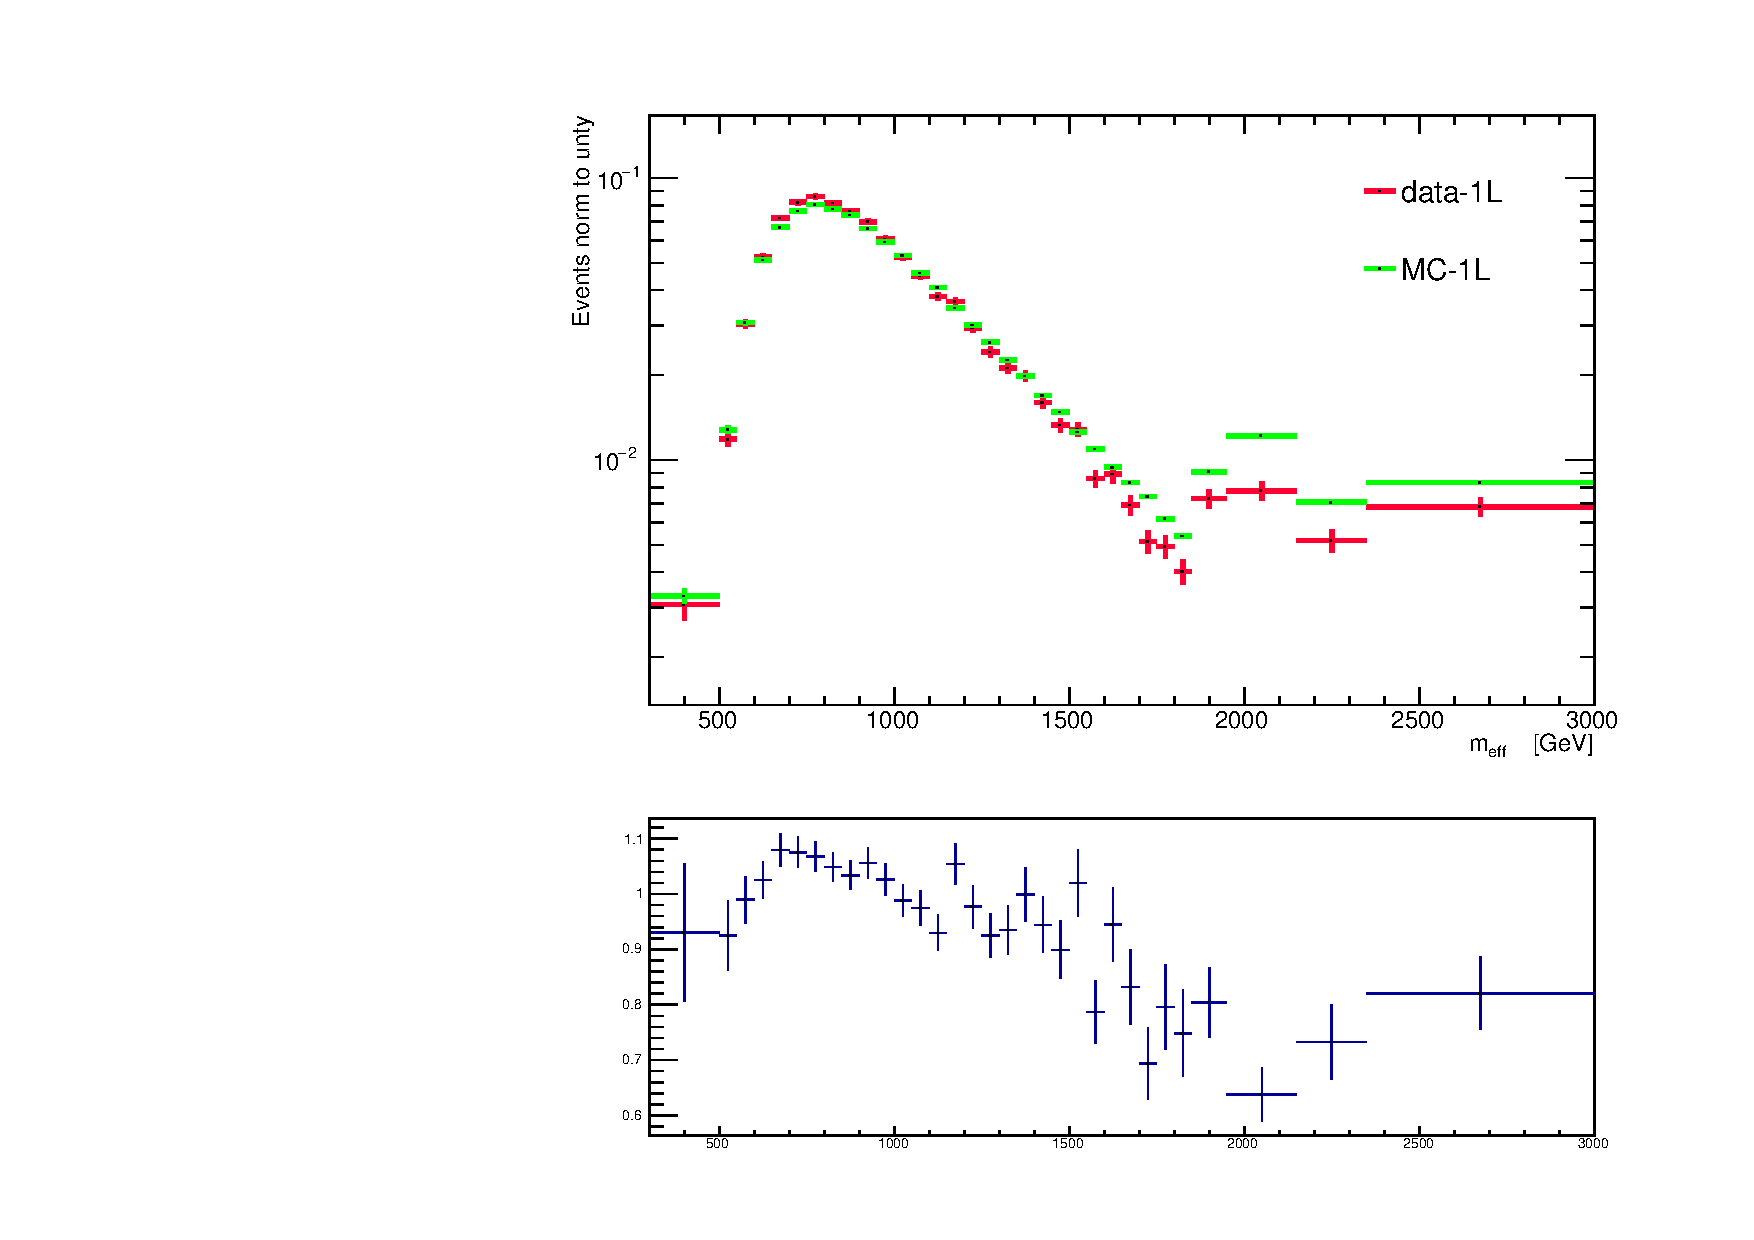
\includegraphics[width=0.55\textwidth]{figures/strong_prod/meff_rw/corr_meff_lowmTb_all_1L.pdf}}
%\subfigure[0L]{\includegraphics[width=0.45\textwidth]{figures/meff_corr/no_meff_corr_2b/meff_incl_Presel_in2b_0l.pdf}}
\caption{$\meff$ distribution in data and MC in a selection that requires exactly 2 b-jets, $\met$ $>$ 200 GeV, $\mtb$ $<$ 140 GeV and
at least one lepton.}
\label{fig:meff_in2b_no_corr}
\end{figure}

